\documentclass{ximera}

%\documentclass{ximera}

\usepackage{float}
\usepackage{subcaption}

\pgfplotsset{compat=1.16}

\newtheorem{ass}{Assumption}

\def\check{\tikz\fill[scale=0.4](0,.35) -- (.25,0) -- (1,.7) -- (.25,.15) -- cycle;}





\outcome{Understand how forward contracts work.}

\author{Brad Waller}

%Section 1.5

\title{Forward Contracts}

\begin{document}

\begin{abstract}
Forward contracts are our first example of a derivative. The beauty of them is that they happen constantly in business!
\end{abstract}

\maketitle

A {\bf forward contract} is one of the most natural examples of a {\bf derivative} that we will see. 

\begin{definition}\label{def20}
A {\bf forward contract}\index{forward contract} is an agreement between two parties, a buyer and a seller. The buyer agrees to pay a specified price for an asset at a specified time. The seller agrees to provide the asset at the specified time.
\end{definition}

\begin{remark}
Other things can be specified in a forward contract. They are private arrangements between individuals, so they are highly unregulated. 
\end{remark}

People are constantly entering into forward contract. Almost all businesses enter into forward contract. A restaurant owner will have to arrange for foods to be delivered to their restaurant. Such arrangements can be made via forward contract. 

You could offer to buy your friend's textbook for a class at the end of the semester, as you plan to take the course next semester. It is likely that your friend would get more by selling to you than they would by selling to the university book store. It is also likely that you would pay less to your friend than you would to the university book store. Both you and your friend are entering into a mutually beneficial contract. 

As it turns out, the contract's dependence on another asset is what makes it a derivative.

\begin{definition}\label{def21}
A {\bf derivative}\index{derivative} is a financial instrument that derives its value from another financial asset. The other financial asset is called the {\bf underlying asset}\index{underlying asset}.
\end{definition}

To determine the price of a derivative, we will need to know the payoff of the derivative. First, we must discuss notation that will frequently be used. 

We will usually have many variables to consider when computing the price of our derivatives. In addition to our underlying asset, we will have the asset's dividend rate, and some risk-free interest rate. Previously, we have seen that the dividend rate would be denoted $\delta$ and the risk-free interest rate is denoted $r$. We will denote the time $t$ price of our underlying asset as $S(t)$. This is also called the time $t$ spot price of the asset. 

The risk-free rate usually comes from a government issued, zero coupon bond. Bonds are issued by governments and businesses to borrow money from the public. If you buy bonds, you are lending money to the issuer. If you sell bonds, you are borrowing money. This distinction will be important whenever we are trying to explain our transactions. The explanations that we provide are just as important as the computations we make.

In addition to the asset, dividend and risk-free rate, there are time variables to consider. Many of the derivatives we deal with are contracts that expire at a particular point in time in the future. We will use $T$ to denote that time of expiration. For variable time, we will use $t$. $s$ will be be used when $t$ has been taken. Let's hope to never need any more time variables. 

There is another variable that we deal with frequently; it is called volatility. We will discuss it in more depth when it becomes necessary. 

Earlier, the importance of computing payoffs of derivatives was stressed. Let's compute some payoffs of a forward contract.

\begin{example}
You wish to become a cattle herder. You will need some land, cows, and corn to feed them (the land you plan to purchase has no grass). You've already arranged your purchase of cows to be in three months. You would like to arrange to buy 10,000 bushels of corn at the same time as you have the cows (you don't want the corn to go bad by buying it today). The price today for corn is \$4/bushel. You agree to pay \$4.15/bushel for the corn in three months to a corn farmer that lives nearby. What is your payoff under the following three scenarios three months from now:
	\begin{enumerate}
	\item the price of corn drops to \$3.85/bushel,
	\item the price of corn rises to \$4.15/bushel,
	\item and the price of corn rises to \$4.70/bushel.
	\end{enumerate}
\end{example}

\begin{solution}
The results differ, but the setup is always the same. Your payoffs are as follows in order.
	\begin{align*}
	10,000(3.85-4.15)&=-3000\\
	10,000(4.15-4.15)&=0\\
	10,000(4.70-4.15)&=5500
	\end{align*}
\end{solution}

The computations seem straight-forward, and that is because they are. In general, the buyer in a forward contract will have a payoff that is equal to
\begin{equation*}
q[S(T)-K]
\end{equation*}
where $q$ is the agreed quantity, $S(T)$ is the price of the underlying asset at expiration, and $K$ is the agreed upon price at expiration. 

The statement "the buyer" in the previous paragraph is important. The seller in the forward contract will always have the opposite payoff diagram. Let's compare them below.


\begin{center}
	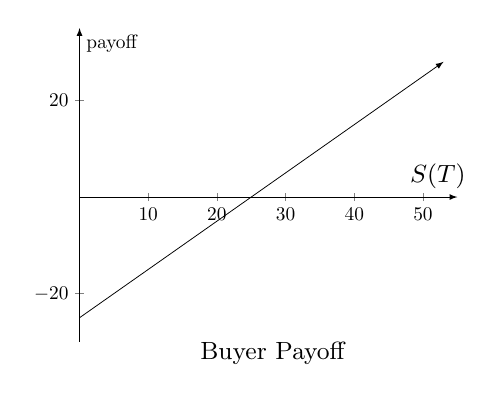
\begin{tikzpicture}[scale=0.7]
		\begin{axis}[
		xmin=0,
		xmax=55,
		%xtick={5,10,...,50},
		ymin=-30,
		ymax=35,
		%ytick={-20,-10,...,50},
		%grid=both,
		axis lines=middle,
		axis line style={->, >=latex},
		x label style={at={(axis description cs:0.86,0.42)},anchor=north},
		%xlabel={$S(T)$},
		ylabel={payoff}]
		%style={font=\tiny}]
		\addplot[black, smooth, domain=0:53, ->, >=latex]{x-25};
		\end{axis}
		\node at (3.5, -0.2){\small Buyer Payoff};
		\node at (6.5, 3){\small $S(T)$};
	\end{tikzpicture}
	\hspace{10pt}
	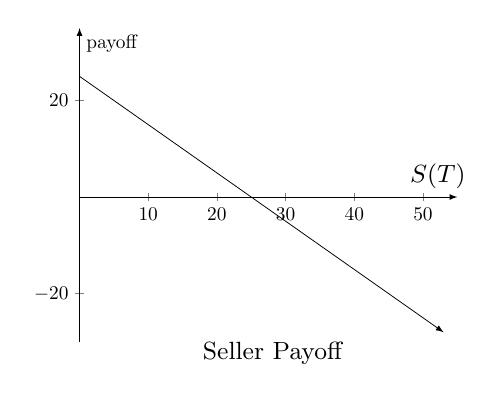
\begin{tikzpicture}[scale=0.7]
	\begin{axis}[
		xmin=0,
		xmax=55,
		%xtick={5,10,...,50},
		ymin=-30,
		ymax=35,
		%ytick={-20,-10,...,50},
		%grid=both,
		axis lines=middle,
		axis line style={->, >=latex},
		x label style={at={(axis description cs:0.86,0.42)},anchor=north},
		%xlabel={$S(T)$},
		ylabel={payoff}]
		%style={font=\tiny}]
		\addplot[black, smooth, domain=0:53, ->, >=latex]{25-x};
	\end{axis}
	\node at (3.5, -0.2){\small Seller Payoff};
	\node at (6.5, 3){\small $S(T)$};
	\end{tikzpicture}
\end{center}

Now that we have the payoffs, we can determine the price of a forward contract. We will need two assumptions to proceed, but first we will need a definition.

\begin{definition}\label{def22}
{\bf Arbitrage} is a type of investment opportunity that carries with it no risk and has a guarantee that the {\bf arbitrageur}\index{arbitrageur} earns a profit. 
\end{definition}

Arbitrage opportunities are usually constructed by matching two payoffs in an advantageous way so that they cancel out. 

\begin{example}
Suppose that you have access to two betting websites. Both give odds on the winner of a game between the Cavaliers and the Lakers. The first site gives the teams equal odds of victory. The second site gives the Cavaliers a 2/3 chance of victory and the Lakers a 1/3 chance of victory. You have \$200 to bet. Determine an arrangement that maximizes your return. The first site will give you a 100\% return on your bet if you choose the correct winner. The second site will pay you a 50\% return if you chose the Cavaliers (and they win) and a 200\% return if you chose the Lakers (and they win). Determine an arbitrage arrangement.
\end{example}

\begin{solution}
One possibility is to bet 110 on the Cavaliers at the first betting site and 90 on the Lakers at the second betting site. The results will be either 220 or 270 (depending on who wins). Since you started with 200, you have made an arbitrage profit!
\end{solution}

\begin{question} Suppose that you have \$200 as in the previous example. How much must you bet with each site so that you always end up with the same amount? What is that amount?
	\begin{prompt}
		\begin{align*}
		&\text{Who do you bet on at the first site?}\answer{Cavaliers}\\
		&\text{Who do you bet on at the second site?}\answer{Lakers}\\
		&\text{What is the value of your bet at the first site?}\answer{120}\\
		&\text{What is the value of your bet at the second site?}\answer{80}\\
		&\text{How much money will you walk away with?}\answer{240}
		\end{align*}
	\end{prompt}
\end{question}

\begin{solution}
You should pick the best odds for each team. This will give you should bet on the Cavaliers at the first site and the Lakers at the second site. Now, the calculation relies on a system of two equations in two unknowns. The first is
	\begin{equation*}
	x+y=200
	\end{equation*}
where $x$ is your bet on the Cavaliers and $y$ is your bet on the Lakers. Using that information, we compute the payoffs from either bet. They would be $2x$ if the Cavaliers win and $3y$ if the Lakers win. We equate these values.
	\begin{equation*}
	2x=3y
	\end{equation*}
Solving this system yields that $x=120$ and $y=80$. This will result in a constant payoff of \$240.
\end{solution}

Now that we have seen how arbitrage works, let's see those two assumptions.

\begin{ass}\label{ass5} Unless a problem is in search of arbitrage, problems will have no arbitrage opportunities.
\end{ass}

\begin{ass}\label{ass6} There will be no fees or taxes unless specified in a problem.
\end{ass}

In the argument to determine the price of a forward contract, we will assume that there are no transaction costs associated with purchases or sales. The idea is to think of a way to end up in the identical payoff position as the buyer in a forward contract. This is not too difficult to do. When you look at the graph of the payoff, you see that there is an axis corresponding to the asset price. In Figure \ref{Fig10}, we had a line with slope 1. In fact, the graph is of the function $S(T)-25$ (for the buyer). In general, this will look like $S(T)-K$. The goal is to come up with a portfolio (collection of assets) that has payoff $S(T)-K$. 

The first position is to enter into a situation where we will end up with one share of the underlying asset at time $T$. The next position is to end up with $-K$ at time $T$. If we borrow money today that is due at time $T$, we will have a negative cash position at time $T$. These two together give us the desired portfolio. Let's use graphs to visualize.

\begin{center}
	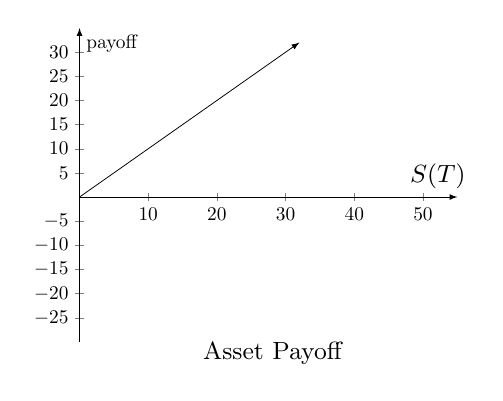
\begin{tikzpicture}[scale=0.7]
	\begin{axis}[
		xmin=0,
		xmax=55,
		%xtick={5,10,...,50},
		ymin=-30,
		ymax=35,
		ytick={-25,-20,...,30},
		%grid=both,
		axis lines=middle,
		axis line style={->, >=latex},
		x label style={at={(axis description cs:0.86,0.42)},anchor=north},
		%xlabel={$S(T)$},
		ylabel={payoff}]
		%style={font=\tiny}]
		\addplot[black, smooth, domain=0:32, ->, >=latex]{x};
	\end{axis}
	\node at (3.5, -0.2){\small Asset Payoff};
	\node at (6.5, 3){\small $S(T)$};
	\end{tikzpicture}
	\hspace{10pt}
	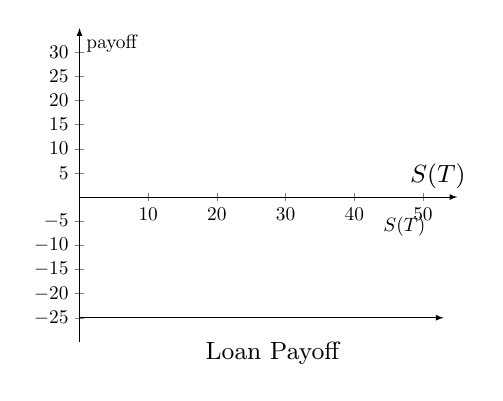
\begin{tikzpicture}[scale=0.7]
	\begin{axis}[
		xmin=0,
		xmax=55,
		%xtick={5,10,...,50},
		ymin=-30,
		ymax=35,
		ytick={-25,-20,...,30},
		%grid=both,
		axis lines=middle,
		axis line style={->, >=latex},
		x label style={at={(axis description cs:0.86,0.42)},anchor=north},
		xlabel={$S(T)$},
		ylabel={payoff}]
		%style={font=\tiny}]
		\addplot[black, smooth, domain=0:53, ->, >=latex]{-25};
	\end{axis}
	\node at (3.5, -0.2){\small Loan Payoff};
	\node at (6.5, 3){\small $S(T)$};
	\end{tikzpicture}
\end{center}

The loan payoff in the figure is negative since we borrowed money at the beginning. That means money will be leaving us at expiration, so its flow is negative. If these two positions are combined, we get the buyer's payoff from earlier. Since there are no other fees or taxes to worry about, we can state our theorem.

\begin{theorem}[Forward Contract Price]\label{thm1}
The time $t$ price of a forward contract to purchase $q$ shares of $S$ for $K$/share that expires at time $T$ is given by the formula
	\begin{equation*}
	q[S(t)e^{-\delta(T-t)}-Ke^{-r(T-t)}].
	\end{equation*}
The time $t$ portfolio that replicates the time $T$ payoff of the forward contract is
	\begin{enumerate}
	\item the purchase of $qe^{-\delta(T-t)}$ shares of the underlying asset and
	\item selling risk-free bonds valued at $qKe^{-r(T-t)}$ today.
	\end{enumerate}
Alternatively, this could be stated 
	\begin{enumerate}
	\item the purchase of $qe^{-\delta(T-t)}$ shares of the underlying asset and
	\item borrowing $qKe^{-r(T-t)}$. 
	\end{enumerate}
\end{theorem}

\begin{remark}
It is important to understand that this price is what the buyer in the contract would have to pay. The situation is reversed for the seller.
\end{remark}

\begin{question}
You enter into a forward contract to purchase 100 shares of ABC in three months for \$75/share. The current price of one share of ABC is \$74. The dividend rate is $\delta=0.03$ and the risk-free rate is $r=0.09$. How much do you pay for the forward contract?
	\begin{prompt}
		\begin{equation*}
		\text{You would pay }\answer{11.57}
		\end{equation*}
	\end{prompt}
\end{question}

\begin{solution}
	This is a direct calculation using the formula provided by Theorem \ref{thm1}. 
	\begin{equation*}
	100[74e^{-0.03/4}-75e^{-0.09/4}]=11.57
	\end{equation*}
\end{solution}	

We can modify the question slightly to see the benefit of having such a formula.

\begin{example}
In one month you decide that you don't want to be involved with purchasing 100 shares of ABC, so you decide to sell your forward contract. The only new condition is that the spot price of ABC has changed to 76. What should you receive for the forward contract?
\end{example}

\begin{solution}	
You should receive
	\begin{equation*}
	100[76e^{-0.03\cdot 2/12}-75e^{-0.09\cdot 2/12}]=173.76.
	\end{equation*}
\end{solution}

\begin{remark}
If we were to enter into a forward contract where the agreed upon price per share is the forward price, then the contract would have no value. We would not need to pay anything for that contract. We could save that quantity today by making a risk-free loan of $qS(t)e^{-\delta (T-t)}$. 
\end{remark}

\begin{definition}
The time $T$ {\bf prepaid forward price} of an asset $S$ at time $t$ is denoted
	\begin{equation*}
	F_{t,T}^P(S).
	\end{equation*}
The value is given by
	\begin{equation*}
	S(t)e^{-\delta(T-t)}.
	\end{equation*}
\end{definition}

Now that we have a way to compute the theoretical price of a forward contract, we would like to use it for practical reasons. This will rely on something called {\bf short selling}, which is the topic of the next section.


\end{document}
